\renewcommand{\mapa}{Poglavja/Slike/grayscale1000}

\begin{figure}[!ht]
    \centering
    \begin{subfigure}{0.49\linewidth}
        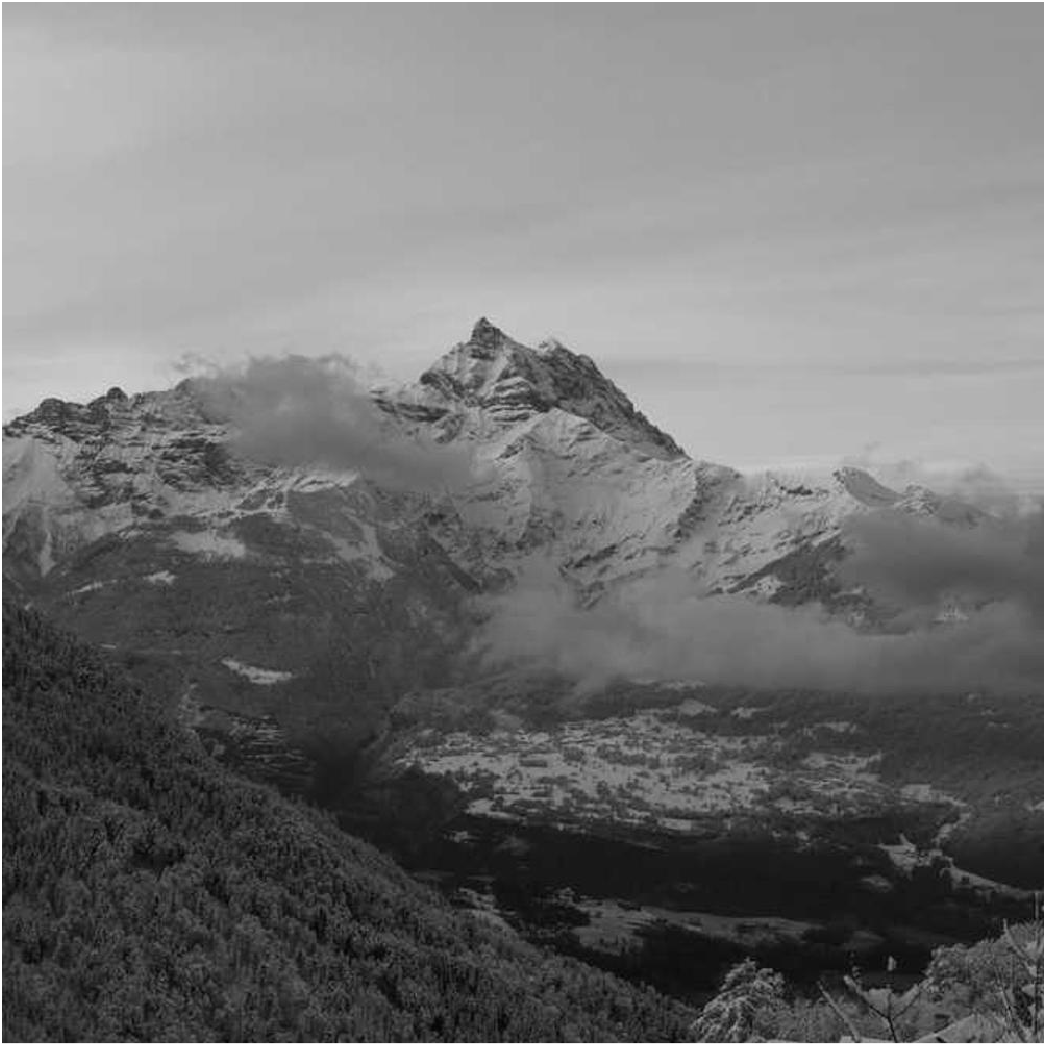
\includegraphics[width=\linewidth]{\mapa/slikaInput.png}
        \caption{Originalna slika.}
    \end{subfigure}
    \hfill
    \begin{subfigure}{0.49\linewidth}
        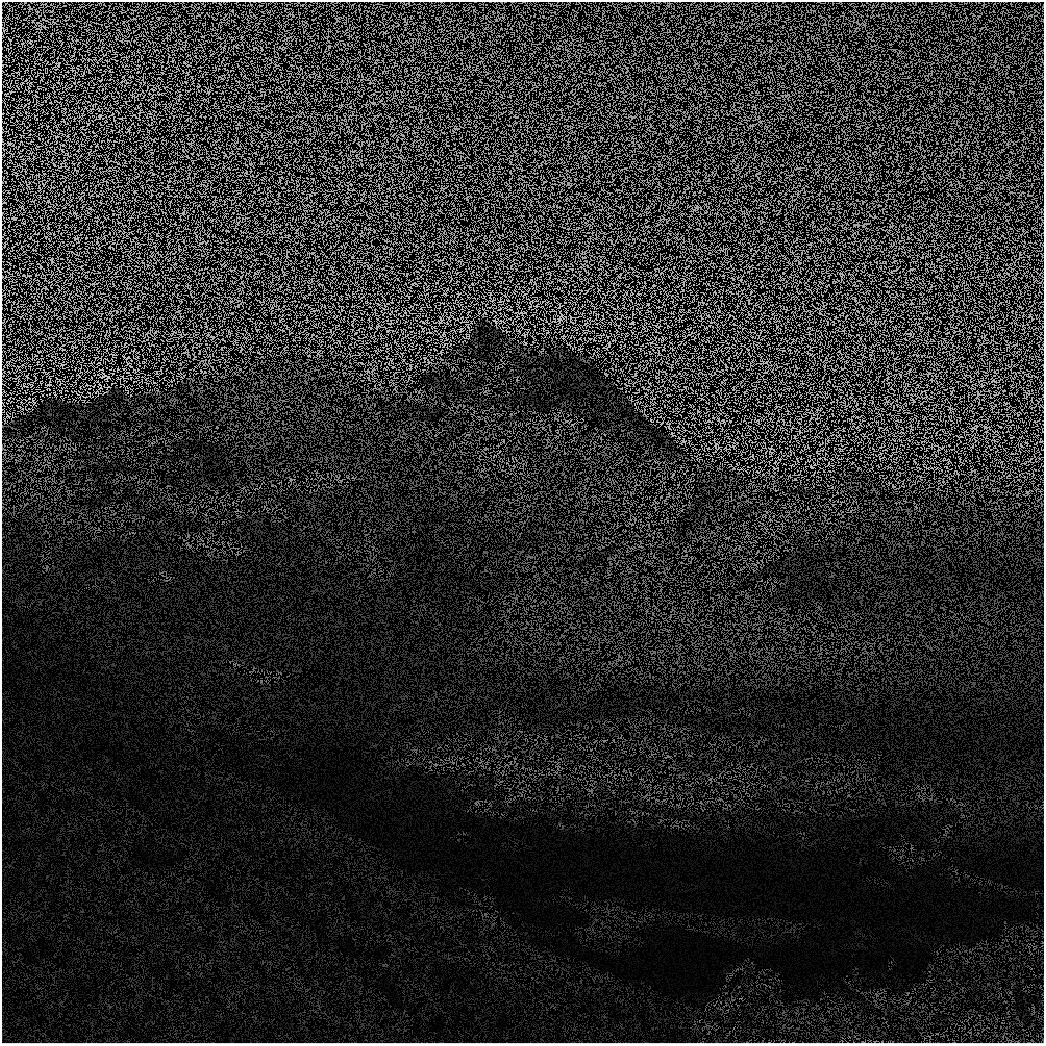
\includegraphics[width=\linewidth]{\mapa/slikaInput35.png}
        \caption{Slika s $35\%$ znanimi podatki.}
    \end{subfigure}
    \begin{subfigure}{0.49\linewidth}
        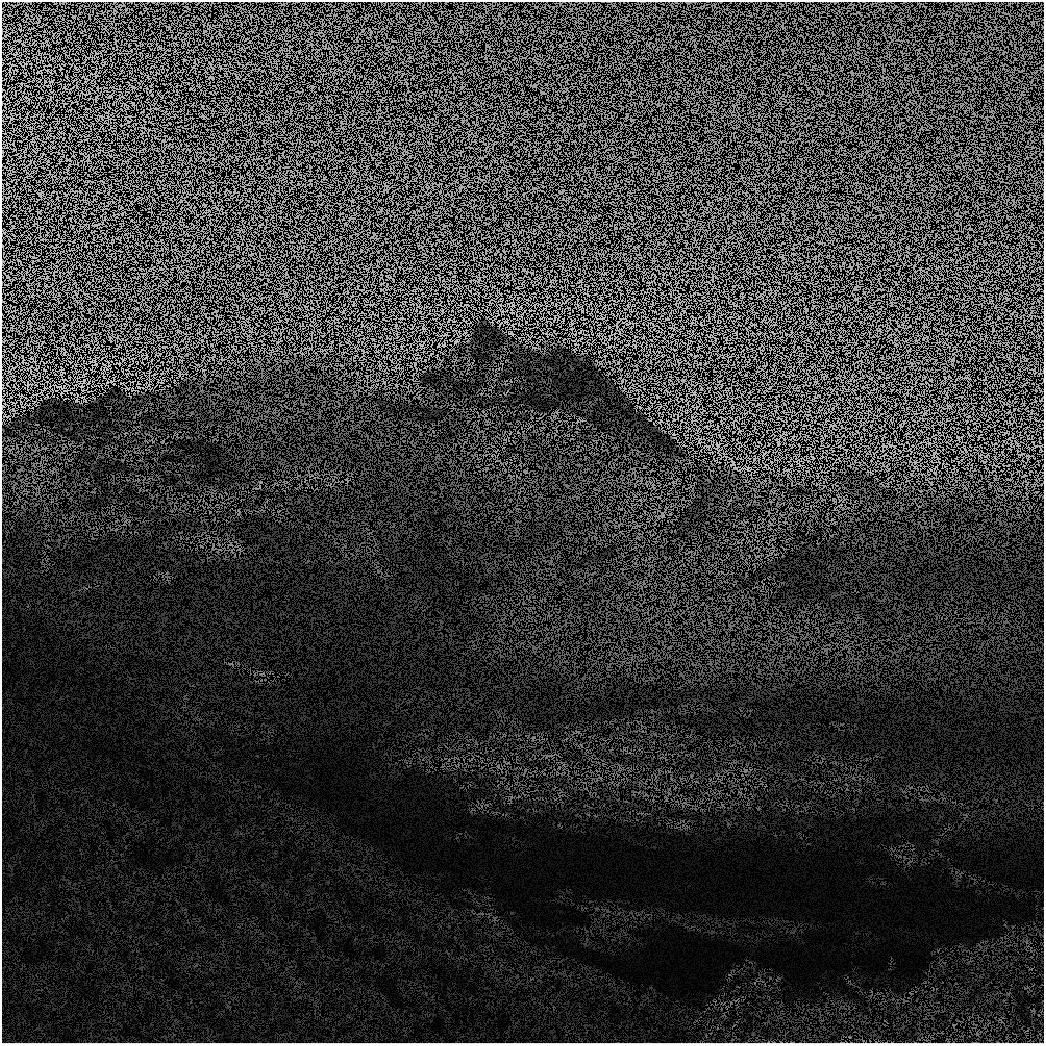
\includegraphics[width=\linewidth]{\mapa/slikaInput45.png}
        \caption{Slika s $45\%$ znanimi podatki.}
    \end{subfigure}
    \hfill
    \begin{subfigure}{0.49\linewidth}
        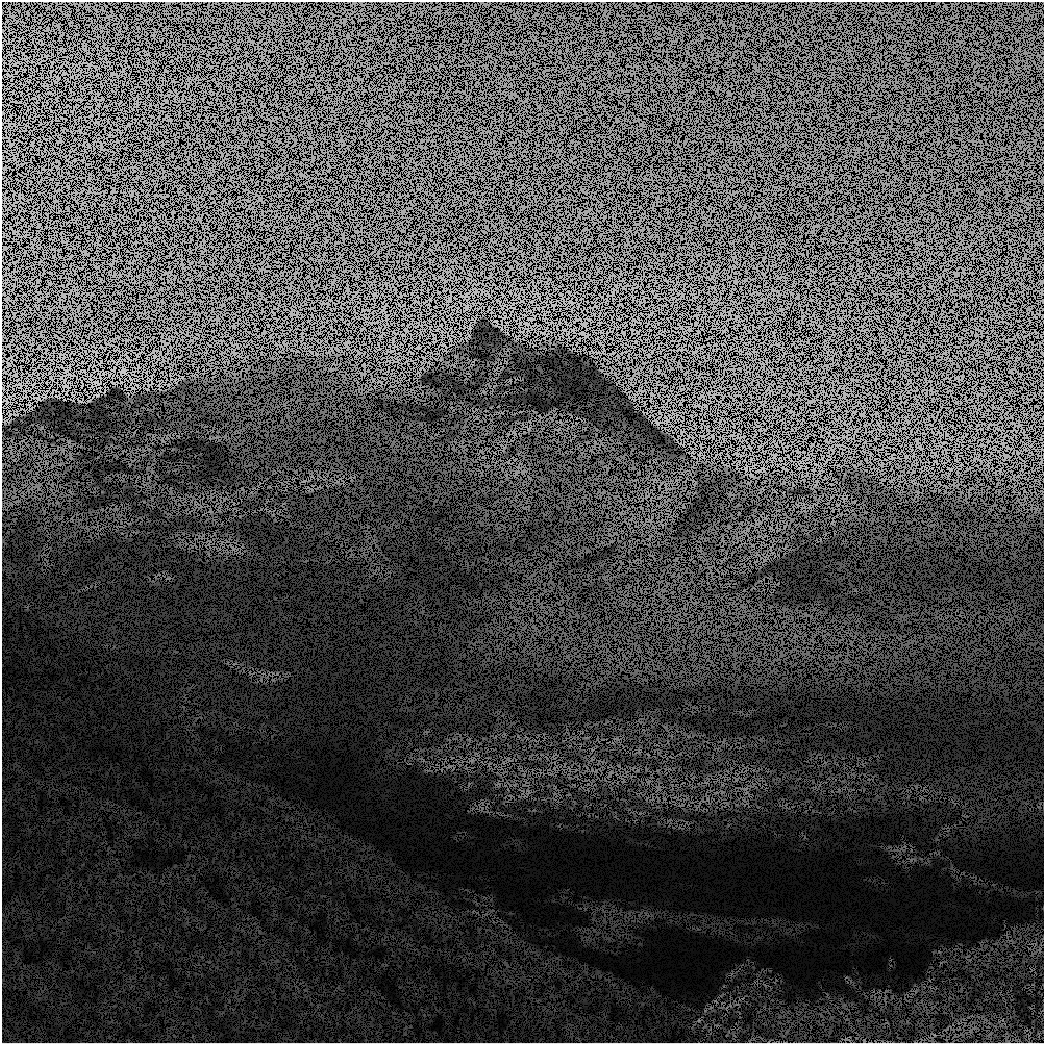
\includegraphics[width=\linewidth]{\mapa/slikaInput60.png}
        \caption{Slika s $60\%$ znanimi podatki.}
    \end{subfigure}
    \caption{Slika, uporabljena za rekonstrukcijo. Vir slike: \cite{UnsplashGora}.}
\end{figure}

\begin{figure}[!ht]
    \centering
    \begin{subfigure}{0.325\linewidth}
        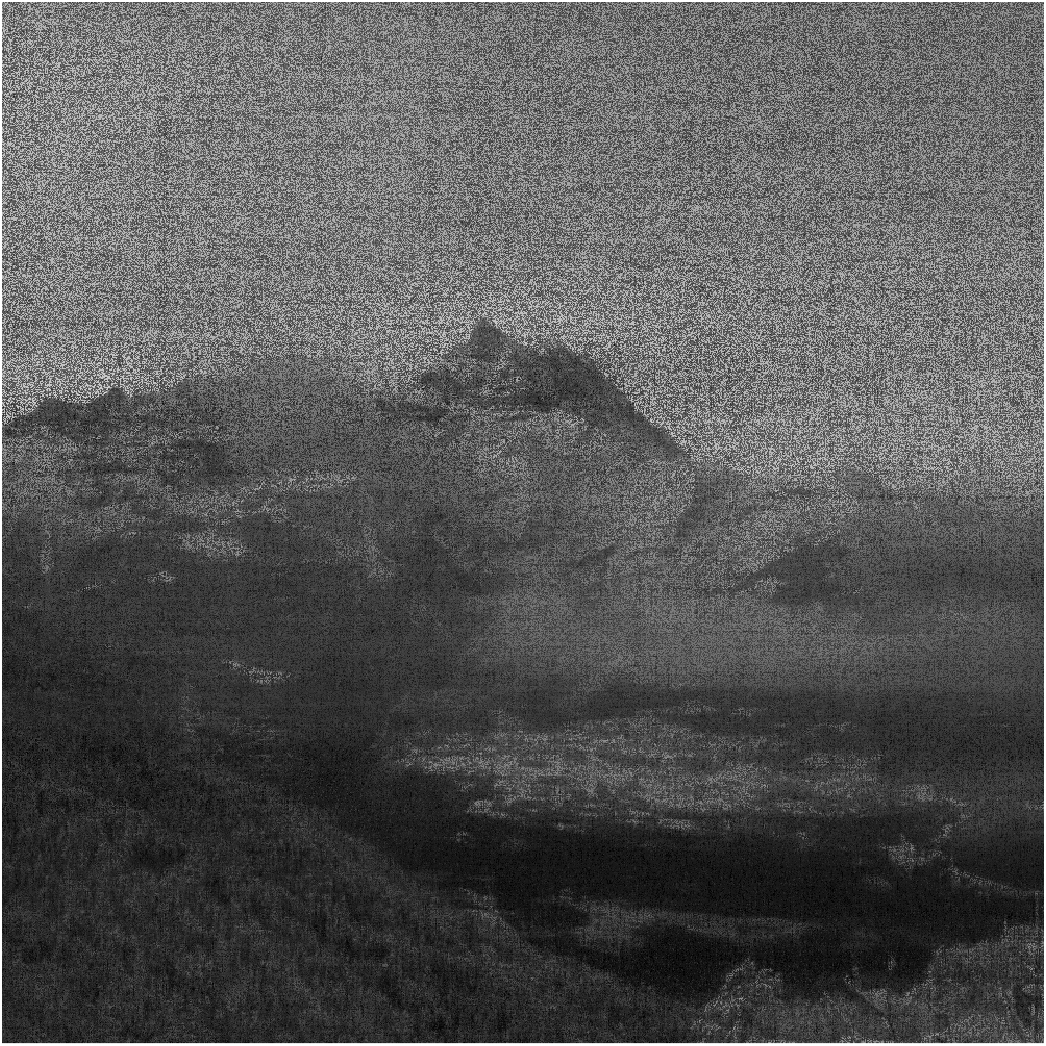
\includegraphics[width=\linewidth]{\mapa/slikaRez35SVT.png}
        \caption{SVT, $35\%$}
    \end{subfigure}
    \hfill
    \begin{subfigure}{0.325\linewidth}
        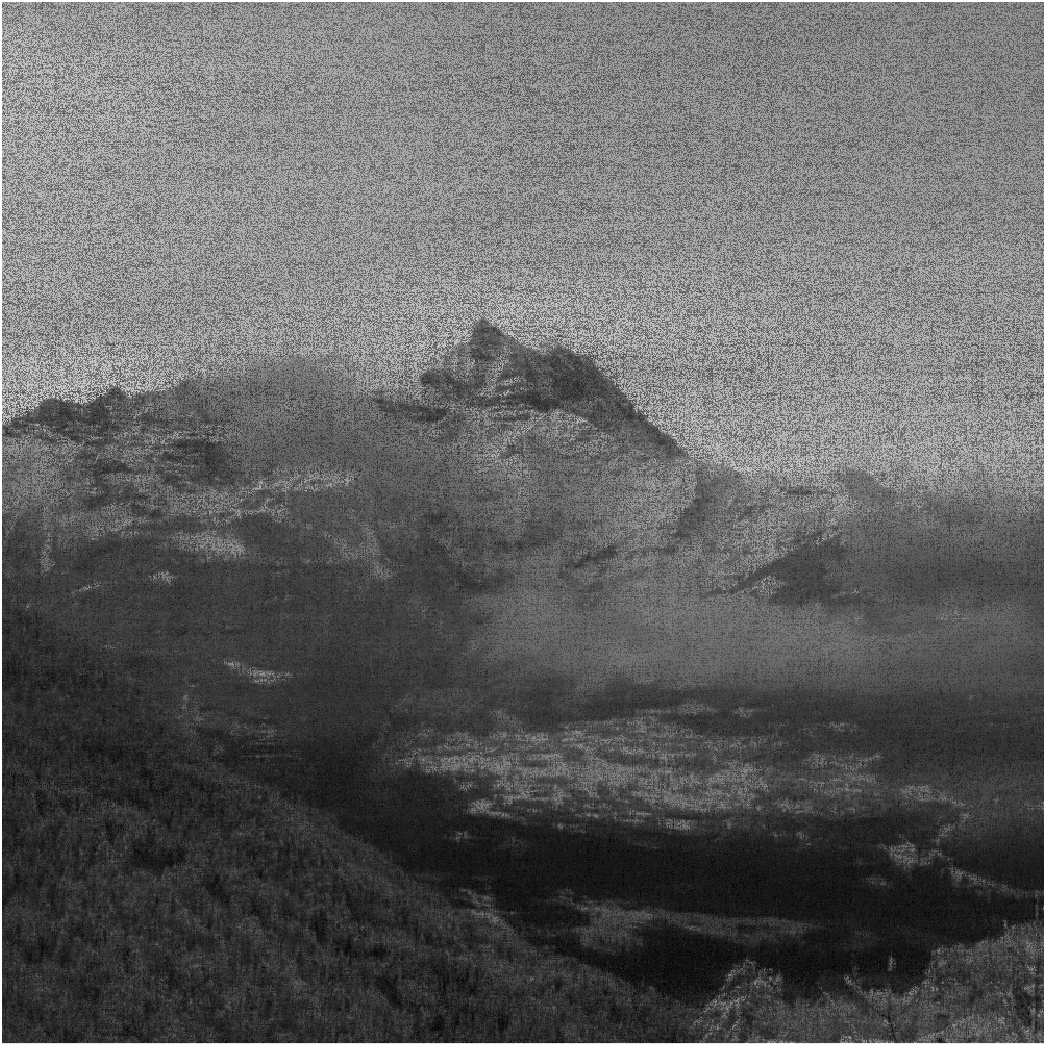
\includegraphics[width=\linewidth]{\mapa/slikaRez45SVT.png}
        \caption{SVT, $45\%$}
    \end{subfigure}
    \hfill
    \begin{subfigure}{0.325\linewidth}
        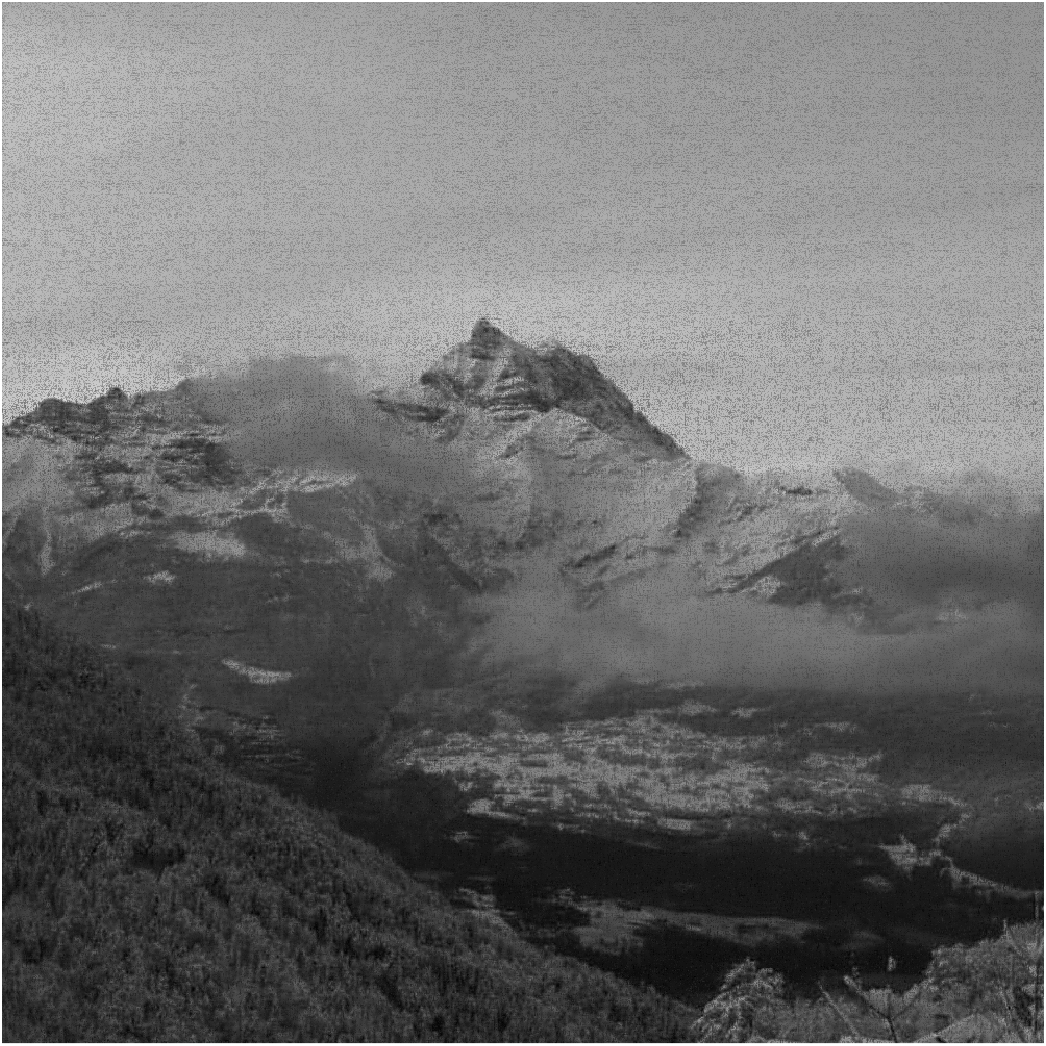
\includegraphics[width=\linewidth]{\mapa/slikaRez60SVT.png}
        \caption{SVT, $60\%$}
    \end{subfigure}
    \begin{subfigure}{0.325\linewidth}
        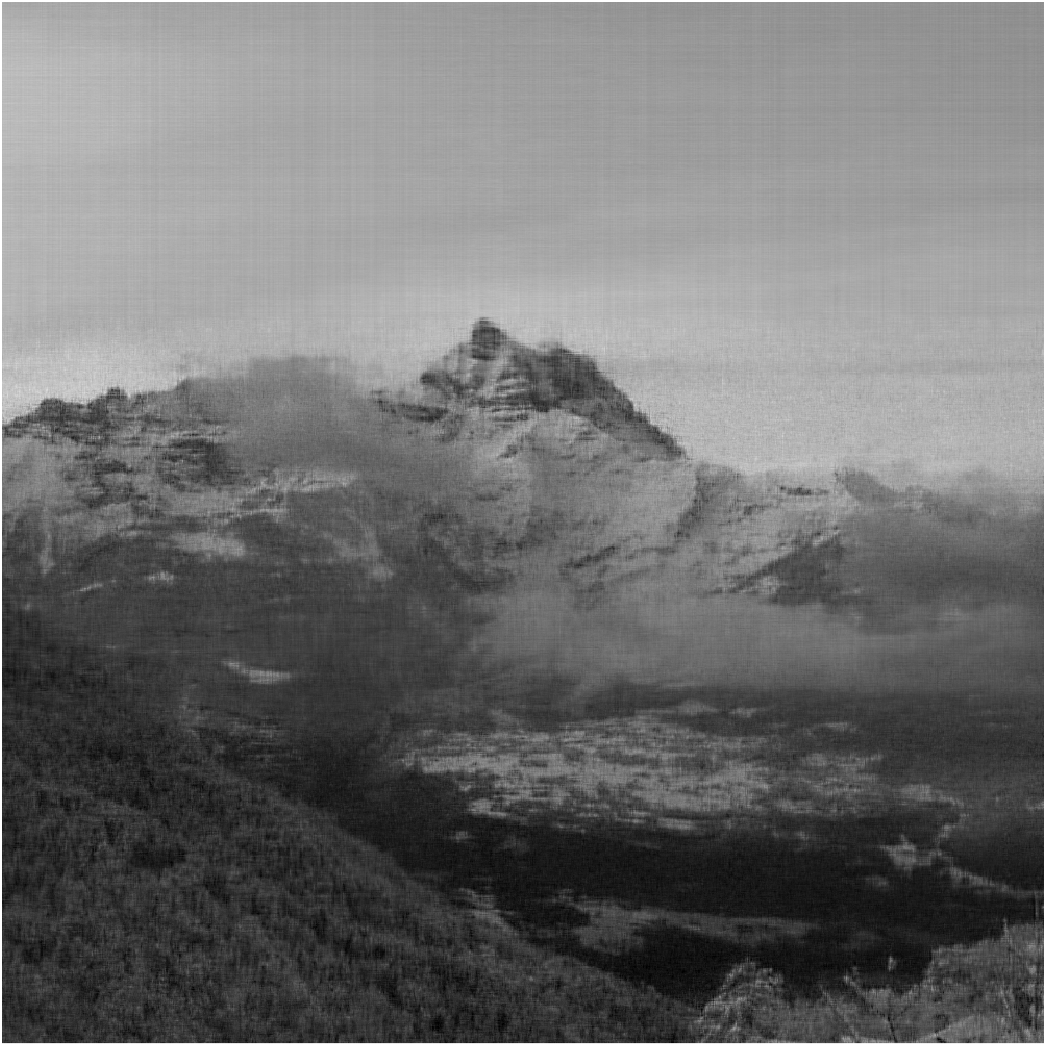
\includegraphics[width=\linewidth]{\mapa/slikaRez35TNNM.png}
        \caption{TNNM, $35\%$}
    \end{subfigure}
    \hfill
    \begin{subfigure}{0.325\linewidth}
        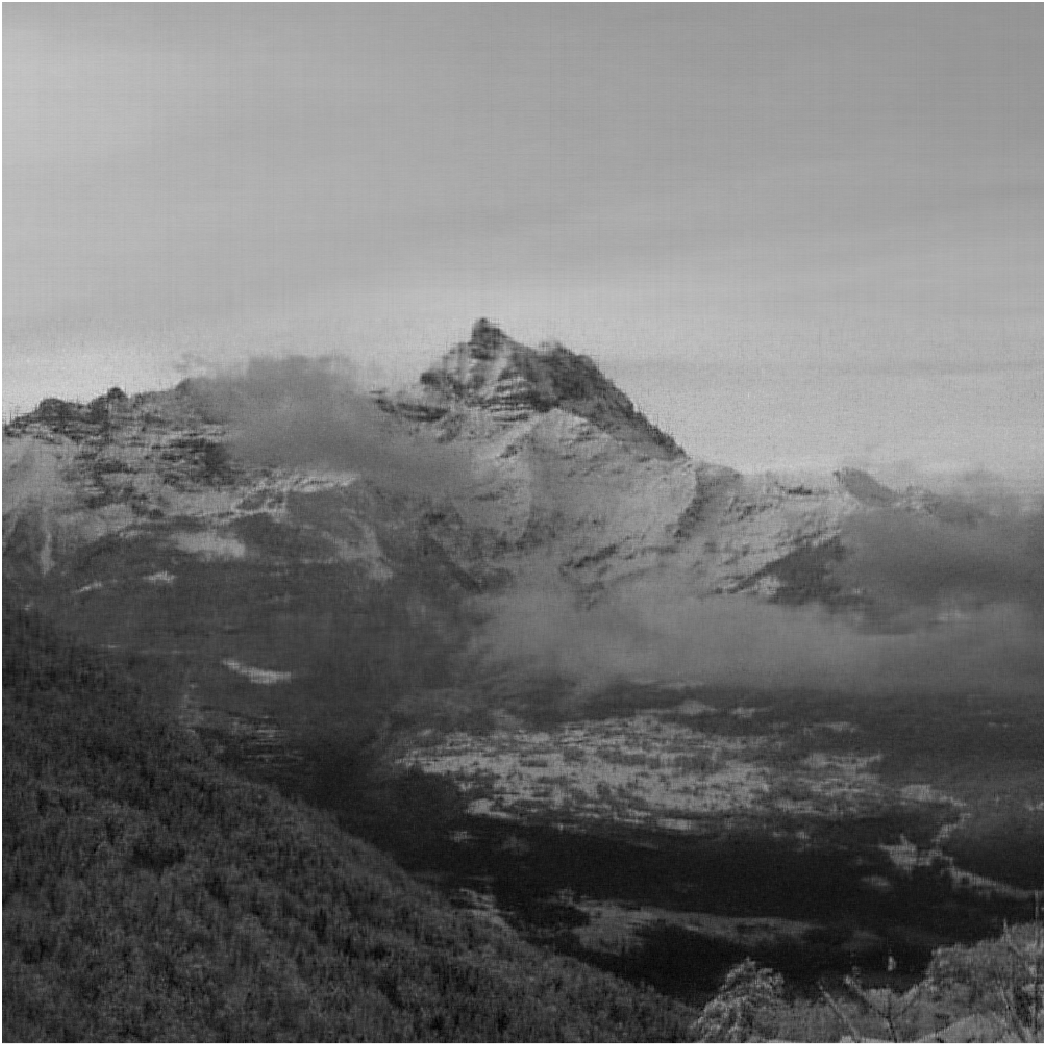
\includegraphics[width=\linewidth]{\mapa/slikaRez45TNNM.png}
        \caption{TNNM, $45\%$}
    \end{subfigure}
    \hfill
    \begin{subfigure}{0.325\linewidth}
        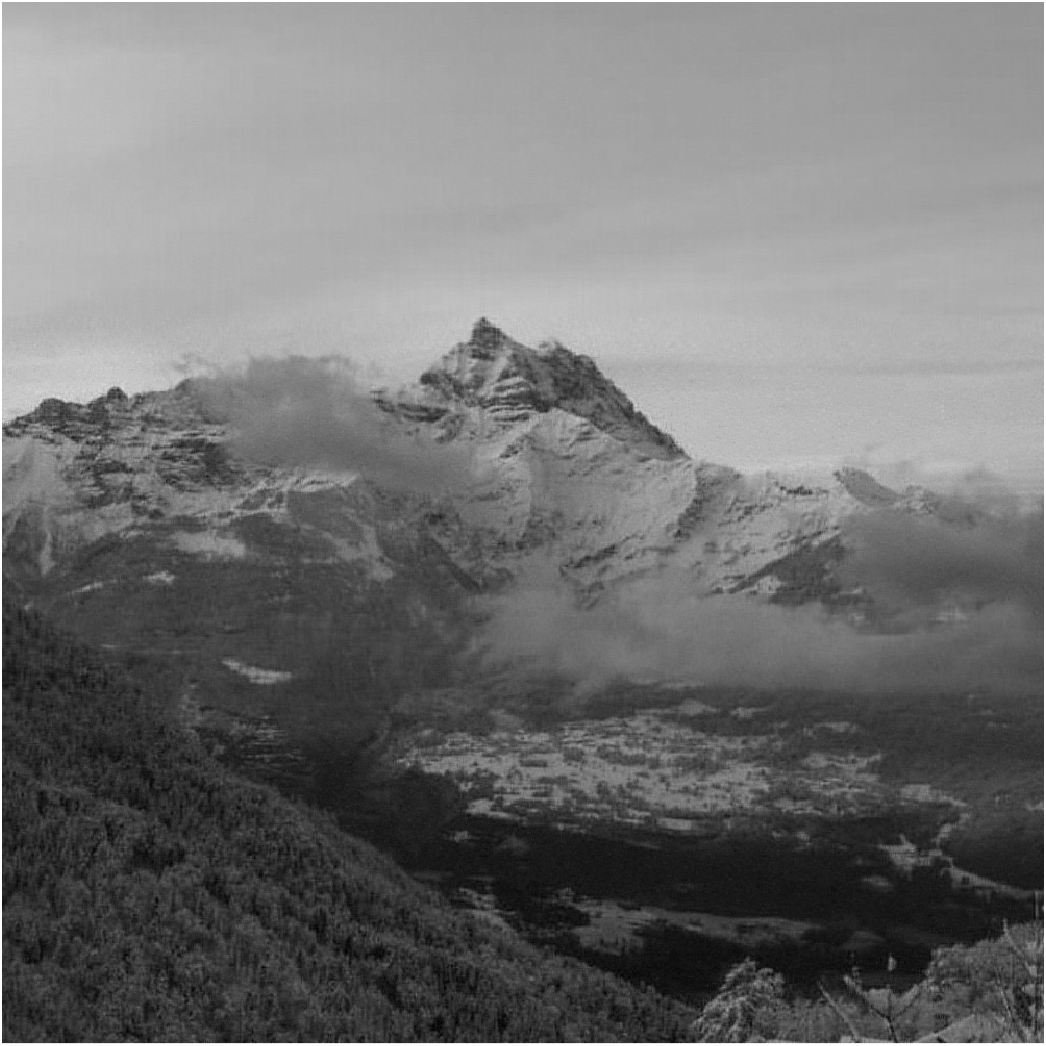
\includegraphics[width=\linewidth]{\mapa/slikaRez60TNNM.png}
        \caption{TNNM, $60\%$}
    \end{subfigure}
    \begin{subfigure}{0.325\linewidth}
        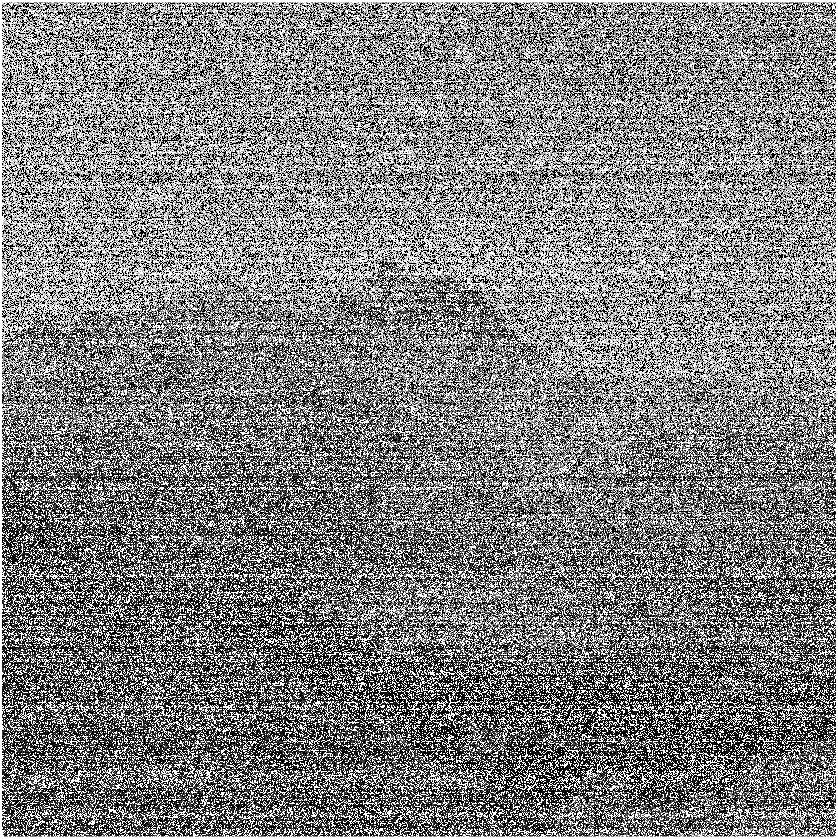
\includegraphics[width=\linewidth]{\mapa/slikaRez35ASD400.png}
        \caption{ASD, $35\%$}
    \end{subfigure}
    \hfill
    \begin{subfigure}{0.325\linewidth}
        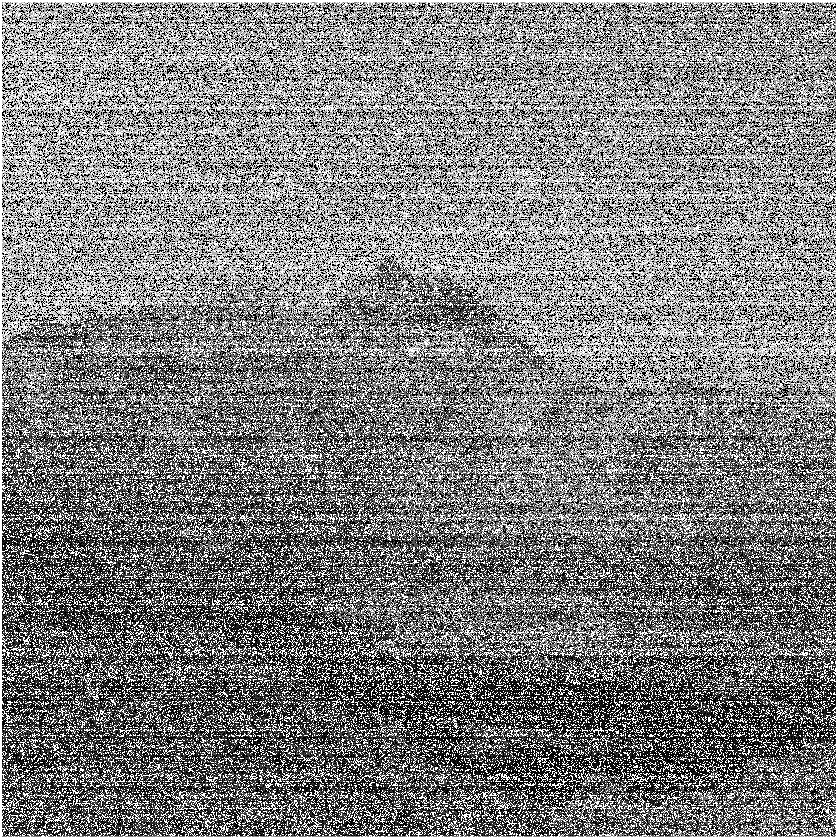
\includegraphics[width=\linewidth]{\mapa/slikaRez45ASD600.png}
        \caption{ASD, $45\%$}
    \end{subfigure}
    \begin{subfigure}{0.325\linewidth}
        %ASD 60?%
        \hfill
    \end{subfigure}
    \begin{subfigure}{0.325\linewidth}
        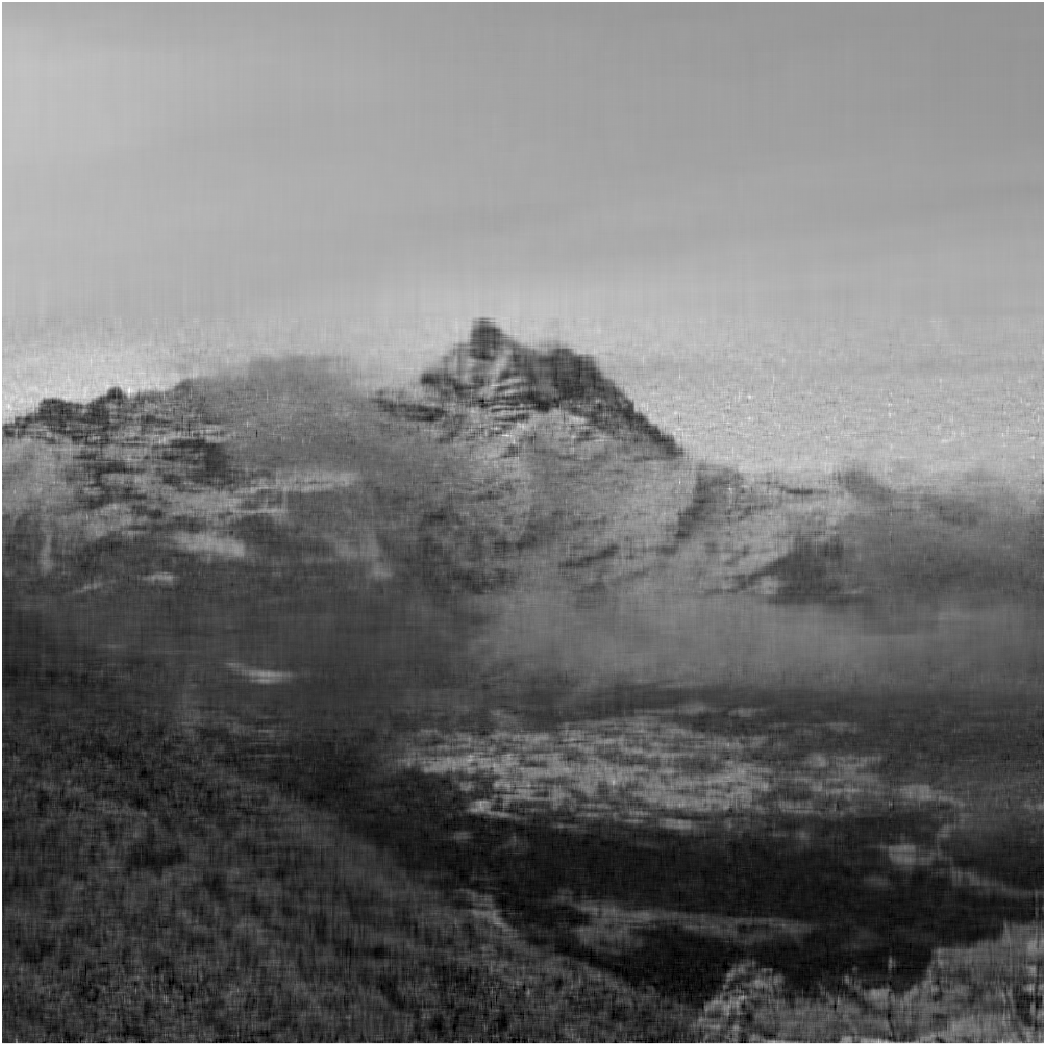
\includegraphics[width=\linewidth]{\mapa/slikaRez35LmaFIT50.png}
        \caption{LMaFit, $35\%$}
    \end{subfigure}
    \hfill
    \begin{subfigure}{0.325\linewidth}
        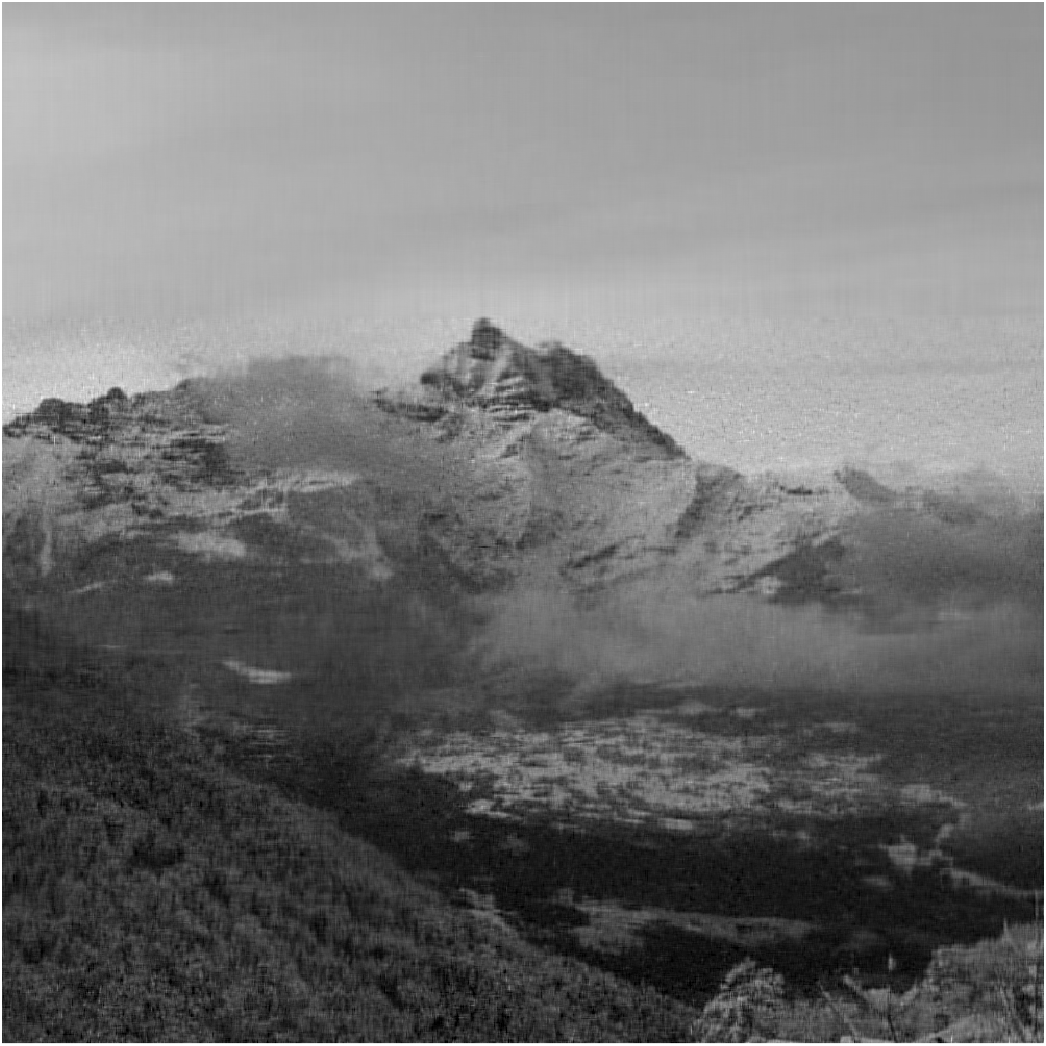
\includegraphics[width=\linewidth]{\mapa/slikaRez45LmaFIT73.png}
        \caption{LMaFit, $45\%$}
    \end{subfigure}
    \begin{subfigure}{0.325\linewidth}
        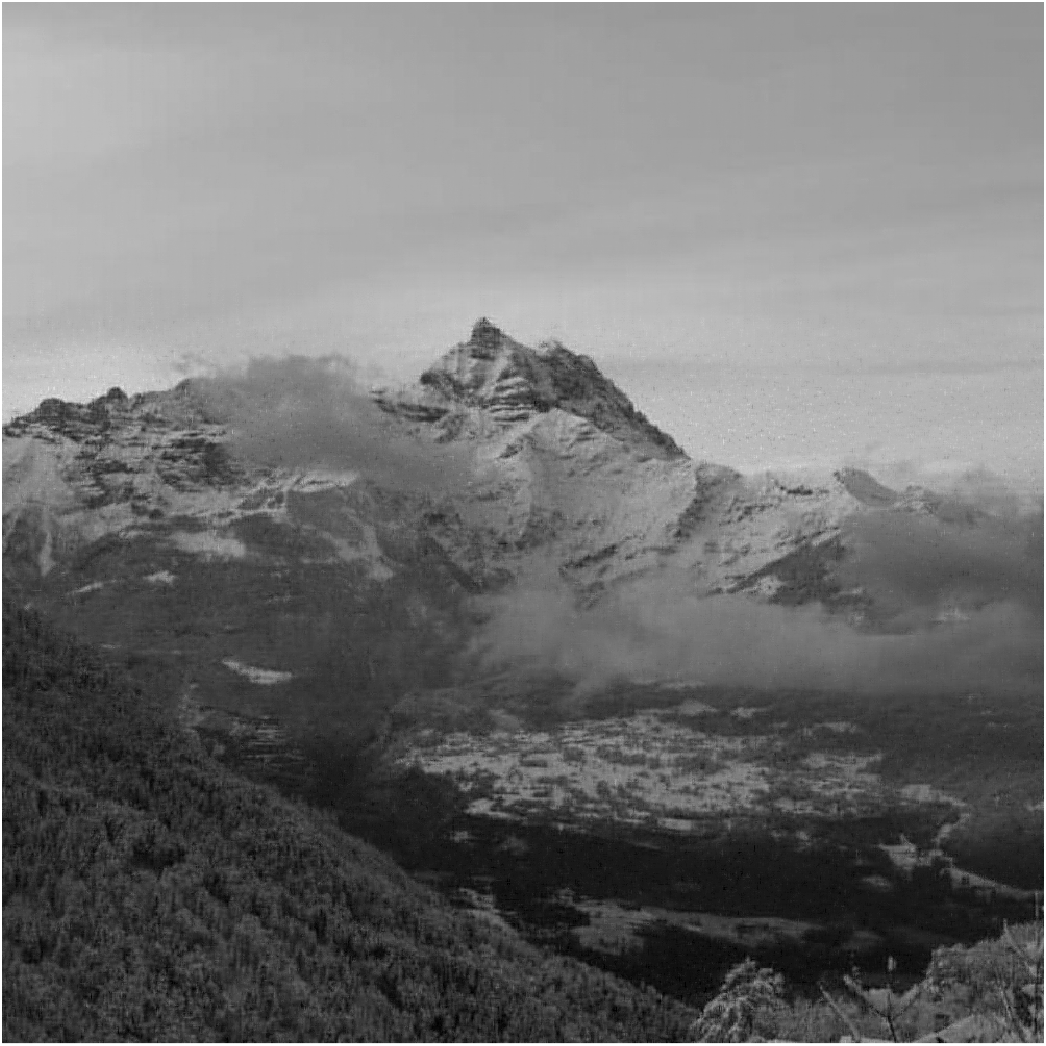
\includegraphics[width=\linewidth]{\mapa/slikaRez60LmaFIT77.png}
        \caption{LMaFit, $60\%$}
    \end{subfigure}
    \caption{Rekonstrukcija zašumljenih slik z uporabo različnih algoritmov in pri različnih odstotkih znanih vrednosti. Kratica pod sliko označuje uporabljen algoritem, odstotek za vejico pa odstotek znanih vrednosti.}
\end{figure}

\FloatBarrier

\begin{table}[h]
    \centering
    \begin{tabular}{|c|c|c|c|c|}
        \hline
        \diagbox{OZP}{Algoritem}
             & SVT                & TNNM               & LMAFIT             & ASD                  \\ \hline
        35\% & $4.69 \times 10^4$ & $7.70 \times 10^3$ & $7.50 \times 10^3$ & $3.97 \times 10^7$ \\ \hline
        45\% & $3.15 \times 10^4$ & $5.30 \times 10^3$ & $5.87 \times 10^3$ & $6.09 \times 10^7$ \\ \hline
        60\% & $1.25 \times 10^4$ & $3.58 \times 10^3$ & $4.20 \times 10^3$ & -                    \\ \hline
    \end{tabular}
    \caption{Napake algoritmov, izračunane v Frobeniusovi normi. Kratica OZP stoji za odstotek znanih podatkov.
    % \CR{Kratico OZP sem umaknil iz seznama uporabljenih kratic. Tam je bolj smiselno dati uveljavljene kratice za algoritme. OZP si sam uvedel in kar v vsako tabeli spodaj dodaj v opis zadnji stavek s pomenom OZP.}
    }
\end{table}
\begin{figure}[!ht]
    \centering
    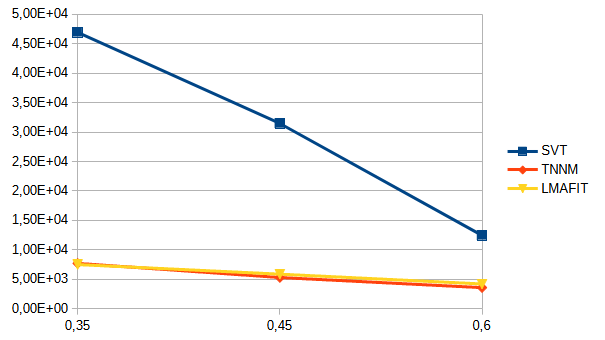
\includegraphics[width=\linewidth]{Poglavja/Slike/grayscale1000/grafNapake.png}
    \caption{Napake algoritmov v Frobeniusovi normi. Na abscisni osi so deleži znanih podatkov slik.}
\end{figure}

\begin{table}[h]
    \centering
    \begin{tabular}{|c|c|c|c|c|}
        \hline
        \diagbox{OZP}{Algoritem}
             & SVT   & TNNM & LMAFIT & ASD   \\ \hline
        35\% & 338s  & 824s & 275s   & 1012s \\ \hline
        45\% & 510s  & 498s & 248s   & 328s  \\ \hline
        60\% & 1674s & 350s & 45.6s  & -     \\ \hline
    \end{tabular}
    \caption{Časi do dosega zaustavitvenega pogoja. Kratica OZP stoji za odstotek znanih podatkov.}
\end{table}
\begin{figure}[!ht]
    \centering
    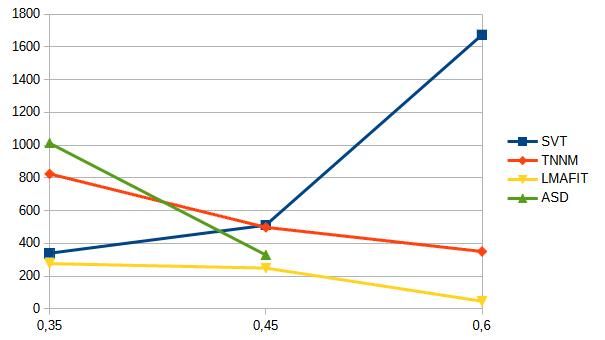
\includegraphics[width=\linewidth]{Poglavja/Slike/grayscale1000/grafCas.png}
    \caption{Časi izvajanja algoritmov. Na abscisni osi so deleži znanih podatkov slik.}
\end{figure}